\section{Rsnap}
\graphicspath{{content/7-solution/3-rsnap/images/}}

\subsection{Interface}
présentation de l'interface :
\begin{itemize}
  \item design joli et adaptative
  \item student side
  \item prof side
  \item arrangement des missions + ouverture successive
  \item passage rsnap/snap
\end{itemize}

\subsection{Implémentation}
Comme expliqué dans la section \ref{Rails}, Rails possède une architecture MVC. Cette section va donc se baser sur sur cette architecture pour présenter la solution proposée.

\subsubsection{modeles}
Les différents concepts utiles pour developper l'application sont ceux représenté par les différents modèles. Ceux-ci sont représenté sur la figure \ref{fig:models}.
%\begin{figure}
%  \begin{center}
%    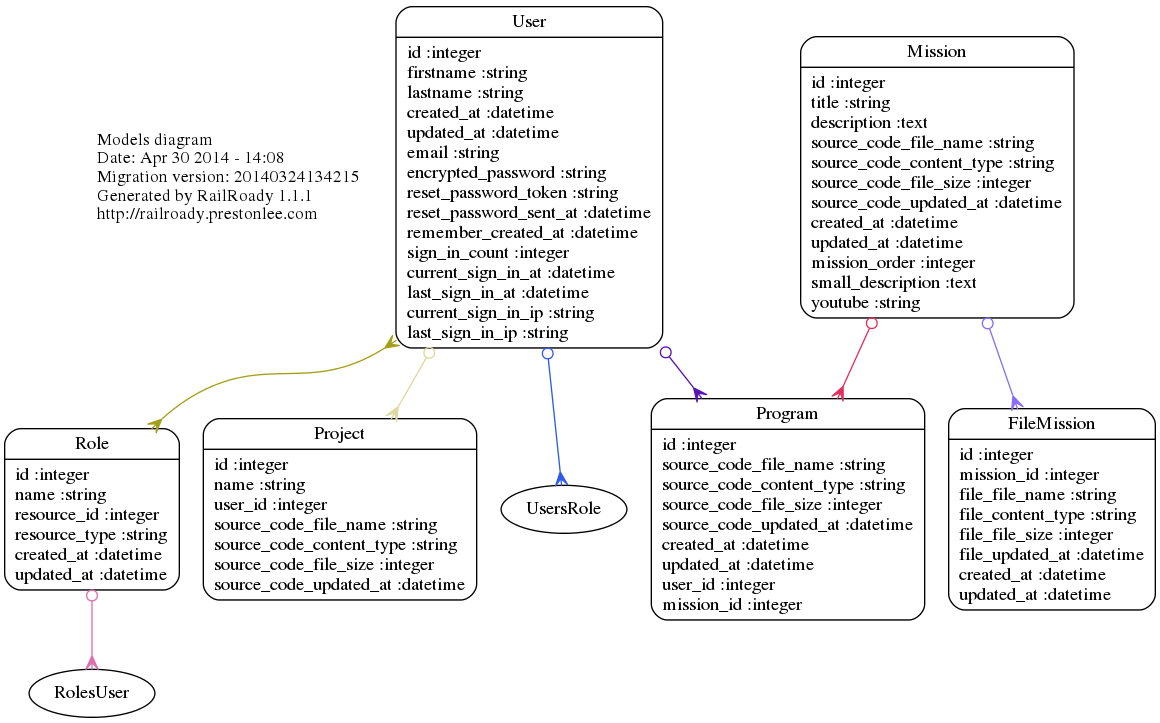
\includegraphics[width=\textwidth]{models_complete}
%    \caption{Modèles de Rsnap}
%    \label{fig:models}
%  \end{center}
%\end{figure}
\paragraph{\texttt{User}} L'utilisateur contient les informations nécessaires à l'utiliser (\texttt{firstname}, \texttt{email} \ldots) et les informations pour s'authentifier (\texttt{encrypted\_password}, \texttt{current\_sign\_in\_ip}, \ldots). L'utilisateur peut posséder plusieurs roles, programmes et projets.
\paragraph{\texttt{Role}} Les rôles permettent de donner des attributs à un utilisateur. Ce modèle a été généré automatiquement par Rolify \ref{role}. Dans le cas de Rsnap, Deux rôles ont été créé : \texttt{admin} et \texttt{teacher}. Ces deux rôles sont globaux et donc ne sont pas rattaché à une ressources spécifique.%TODO dans future work: role teacher sur ressource students_group

Les roles seront utiles en conjontion avec les autorités \ref{authority} pour donner des droits supplémentaires à ces type d'utilisateurs.
\paragraph{\texttt{Mission}} Les missions représentent tout ce qui est nécessaire pour avoir un exercice. Un mission comporte donc un titre, une description avec des images et une vidéo pour expliquer à l'étudiant ce qu'il devra faire. Elle comporte en plus le code source initial de l'exercice. Généralement, celui-ci contient les squelette initial du programme pour l'étudiant et les tests pour vérifier le programme. 
\paragraph{\texttt{FileMission}} Les fichiers lié à une mission sont les différentes images que compose la description. %TODO dans furture work : on peut imaginer rajouter la possibiliter de mettre d'autres style de fichier dedans : ex. pdf, slide de cours...
\paragraph{\texttt{Program}} Les programmes comportent les solutions des étudiants à une mission donnée. Il comporte uniquement le code source de l'étudiant.
\paragraph{\texttt{Project}} Les projets sont identique à un programme excepté qu'ils ne sont pas lié à une mission. Il comporte donc le nom du projet en plus du code source.

\paragraph{Exemple} \texttt{Program} est un bon exemple de modèle Rails (code source \ref{lst:model-program}). Seul les fonctionnalités que Active Record \ref{active-record} ne sait pas déduire de lui-même sont présentes. Le modèle contient donc uniquement :
\begin{itemize}
  \item le nom des modèles avec qui il est associé et la cardinalité de la relation (\texttt{belong\_to}) ;
  \item la validation de certains attributs pour qu'ils respectent certaines contraintes (\texttt{validate}) ;
  \item des méthodes de classes pour simplifier les requêtes au modèle (\texttt{scope}, \texttt{self.*}).
\end{itemize}

Comme c'est visible dans les \texttt{scope}, Active Record permet de faire des requêtes SQL directement en Ruby. 
%\lstinputlisting[language=Rails, firstline=21, caption={Modèle \texttt{Program}}, label=lst:model-program]{content/7-solution/3-rsnap/program.rb}

\subsubsection{Controlleurs}
Les contrôleurs donnent accès à différentes ressources. La figure \ref{fig:controllers} montre la liste des contrôleurs implémenté pour l'application. La majorité de ceux-ci se rapporte directement à un modèle spécifique. Il existe néanmoins certaines ressources différentes tel que : 
\begin{itemize}
  \item les pages statiques (\texttt{HomeController}) ;
  \item l'ordonnancement des missions (\texttt{SortMissionsController}) ; 
  \item la création d'un programme depuis une mission (\texttt{InitializationMissionController}) ;
  \item les ressources utile à l'affichage de Snap! (\texttt{SnapAssetsController}).
\end{itemize}
%\begin{figure}
%  \begin{center}
%    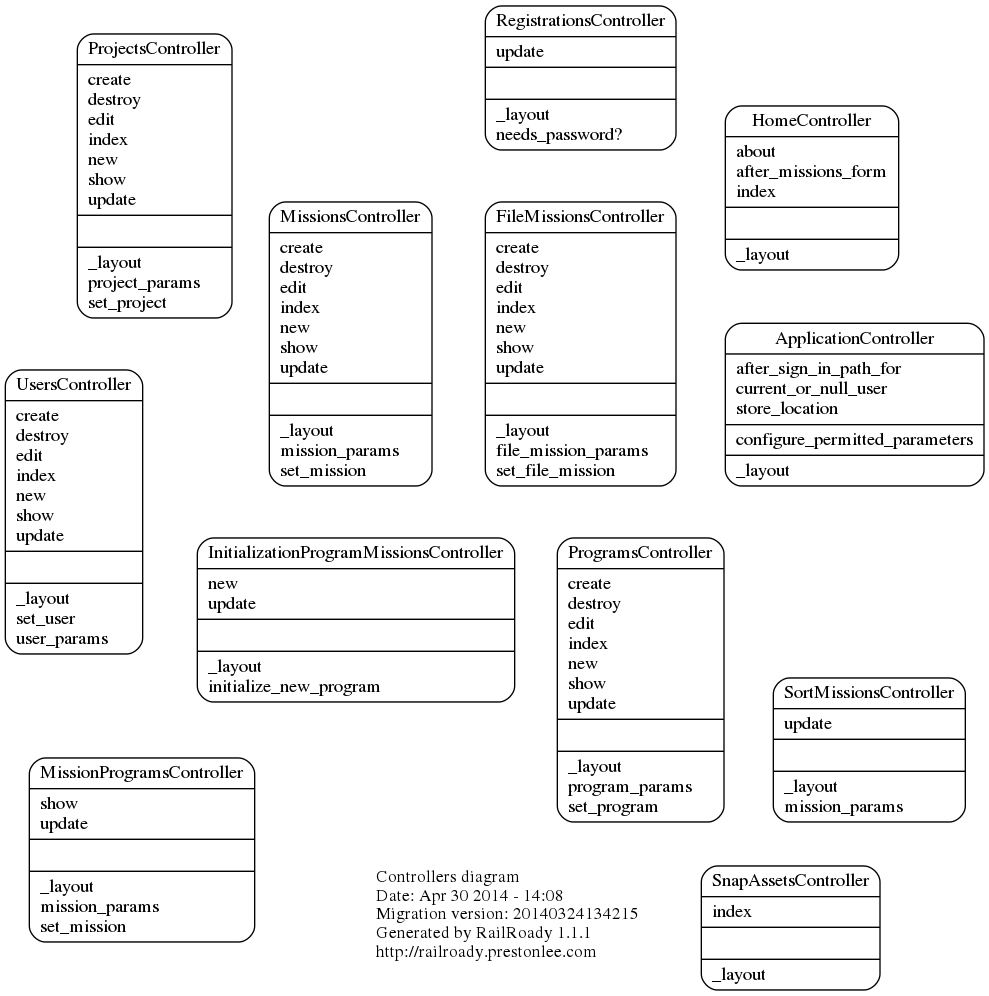
\includegraphics[width=\textwidth]{controllers_complete}
%    \caption{Controlleurs de Rsnap}
%    \label{fig:controllers}
%  \end{center}
%\end{figure}

Comme expliqué dans la section \ref{controller}, les méthodes accessibles sont définie dans \texttt{routes.rb}. Les controlleurs ont des tous des ressources RESTfull excepté \texttt{HomeController}. Ceci est visible dans \texttt{routes.rb} ou en regardant les fonctions publiques disponible dans les controlleurs sur la figure \ref{fig:controllers}.

\paragraph{Exemple}
L'extrait du controlleur \texttt{MissionsController} \ref{lst:controller-mission} montre l'usage classique d'un controlleur. 

%\lstinputlisting[language=Rails, linerange={1-5,10-34,52-62}, caption={Extrait du controlleur \texttt{MissionsController}}, label=lst:controller-mission]{content/7-solution/3-rsnap/missions_controller.rb}

Grâce à la métaprogrammation, \lstinline[language=Rails]{authorize_actions_for Mission} permet de rajouter, sur toutes les méthodes RESTfull, une vérification de ce que peut réaliser ou pas l'utilisateur courant. Ces vérifications sont déportée dans les autorités \ref{autority}. De plus, la méthode \lstinline[language=Rails]{before_filter} permet de réaliser une action supplémentaire avant chaque appel de fonction. Ici, excepté pour l'action \texttt{show} et \texttt{index} qui peuvent être publique, il faut que l'utilisateur soit authentifié pour que l'application puisse par après vérifier ses droits.

Dans une méthode du contrôleur accessible via les routes, plusieurs actions sont à réaliser :
\begin{enumerate}
  \item Traiter si nécessaire les paramètres fournis. Ceux-ci se trouve dans \lstinline[language=Rails]{param} ;
  \item Assigner les variables d'instance que nécessitera la vue pour s'afficher correctement ;
  \item Exécuter le rendu de la page. Si la vue a le même nom que la méthode, cette étape est facultative.
\end{enumerate}

\subsubsection{Vue}
Les vues sont écrite en haml \ref{haml}. L'exemple de code \ref{lst:vue-user-index} avec \ref{lst:vue-user-partial} montre comment est représenté la vue servant à lister tout les utilisateur \ref{fig:vue-users}.

%\lstinputlisting[language=haml, caption={Vue \texttt{index} des utilisateurs}, label=lst:vue-user-index]{content/7-solution/3-rsnap/index.html.haml}
Le code source \ref{lst:vue-user-index} présente comment sont utilisé les variables d'instance créées par le controlleur. Par exemple, la variable \texttt{@title} sert de titre 1.

%\lstinputlisting[language=haml, caption={Vue d'une ligne \texttt{\_user} représentant un utilisateur}, label=lst:vue-user-partial]{content/7-solution/
De plus, Rails permet de faire le rendu d'un autre fichier de manière élégante. La ligne 14 du code source \ref{lst:vue-user-index} permet d'exécuter le rendu sur tout les éléments de la collection \texttt{users} grâce au fichier \ref{lst:vue-user-partial}

Les connaisseurs de Bootstrap \ref{bootstrap} auront reconnu l'usage intensif des classes de style qu'il propose. L'adaptativité de cet outil est visible sur la capture d'écran \ref{fig:vue-users}. En effet, le menu supérieur à été minifié car la taille de l'écran était trop petite pour acceuillir le menu en entier.

\begin{figure}
  \begin{center}
    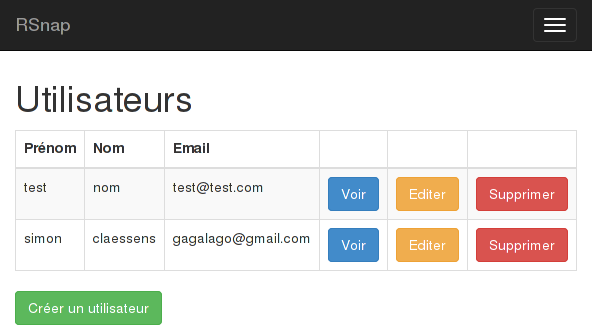
\includegraphics[width=.8\textwidth]{users}
    \caption{Affichage de la vue présentée par le code source \ref{lst:vue-user-index} et \ref{lst:vue-user-partial}}
    \label{fig:vue-users}
  \end{center}
\end{figure}

\subsection{Choix tecniques}
expliquer les différentes possibilité de stockage(fichier et site) prix, fonctionnalité...
